\chapter{Algebraic Geometry}
A summary to a course on an introduction to sheaf cohomology. We will
mostly reference Donu's notes available here
\url{https://www.math.purdue.edu/~dvb/classroom.html}, but also cite Ravi
Vakil's \emph{Fundamentals of Algebraic Geometry} \cite{vakil} available
here \url{https://math216.wordpress.com/}.

\section{The statement of de Rham's theorem}
These are almost verbatim Arapura's notes on the de Rham Complex and
cohomology.

Before doing anything fancy, let's start at the beginning. Let
\(U\subseteq\bbR^3\) be an open set. In calculus class, we learn about
operations
\[
  \{\,\text{functions}\,\}
  \xrightarrow{\,\nabla\,}
  \{\,\text{vector fields}\,\}
  \xrightarrow{\,\nabla\times\,}
  \{\,\text{vector fields}\,\}
  \xrightarrow{\,\nabla\cdot\,}
  \{\,\text{functions}\,\}
\]
such that \((\nabla\times)(\nabla)=0\) and
\((\nabla\cdot)(\nabla\times)=0\). This is a prototype for a
\emph{complex.} An obvious question: does \(\nabla\times v=0\) imply that
\(v\) is a gradient? Answer: sometimes yes (e.g.\@ if \(U=\bbR^3\)) and
sometimes no (e.g.\@ if \(U=\bbR^3\) minus a line). To quantify the failure
we introduce the first de Rham cohomology
\[
  H_{\dR}^1(U)=\frac{\bigl\{\,\text{\(v\) a vector field on
      \(U\)}:\nabla\times v=0\,\bigr\}}{\bigl\{\,\nabla f\,\bigr\}}.
\]
Contrary to first appearances, for reasonable \(U\) this is finite
dimensional and computable. This follows from the de Rham's theorem, which
we now explain. First, let's generalize this to an open set
\(U\subset\bbR^n\). Once \(n>3\) vector calculus is useless, but there is a
good replacement. A differential form of degree \(p\), or \(p\)-form, is an
expression
\[
  \alpha=\sum f_{i_1,\dotsc,i_p}(x_1,\dotsc,x_n)\diff
  x_{i_1}\wedge\dotsb\wedge dx_{i_p}
\]
such that the \(x_i\) are coordinates, the \(f\) are \(C^\infty\)
functions, \(dx_{i_1}\wedge\dotsb\wedge dx_{i_p}\) are symbols where
\(\wedge\) is an anticommutative product. Let \(\calE^p(U)\) denote the
vector space of \(p\)-forms. Define the exterior derivative by
\[
  d\alpha=\ssum_j\frac{\partial f_{i_1,\dotsc,i_p}}{\partial
    x_j}\diff x_j\wedge\dotsb\wedge dx_{i_p}.
\]
This is a \((p+1)\)-form.

\begin{lemma}
  \(d^2=0\).
\end{lemma}
\begin{proof}
  We prove it for \(p=0\). In this case, we have
  \begin{align*}
    df&=\sum_i\frac{\partial f}{\partial x_i}\diff x_i\\
    d(df)&=\ssum_{i,j}\frac{\partial^2}{\partial x_j\partial x_i}\diff
           x_j\wedge dx_i.
  \end{align*}
  Using anticommutativity, we can rewrite this as
  \[
    \sum_{j<i}\left(\frac{\partial^2 f}{\partial x_j\partial x_i}
    -\frac{\partial^2 f}{\partial x_i\partial x_j}\right) dx_j\wedge dx_i=0.
  \]
\end{proof}

A cochain complex is a collection of Abelian groups \(M^i\) and
homomorphisms \(d\colon M^i\to M^{i+1}\) such that \(d^2=0\). We define the
\(p\)\textsup{th} cohomology of this by
\[
  H^p_\dR(M^\bullet,d)=\frac{\Ker d\colon M^p\to M^{p+1}}{\Img d\colon
    M^{p-1}\to M^p}.
\]
So we have an example of a complex \((\calE^\bullet(U),d)\) called the de
Rham complex of \(U\). It's cohomology is the de Rham cohomology
\(H_{\dR}^p(U)=H^p\bigl(\calE^\bullet(U),d\bigr)\). Here is a basic
computation.

\begin{theorem}[Poincaré's lemma]
  \[
    H_{\dR}^p(\bbR^n)=
    \begin{cases}
      \bbR&\text{if \(p=0\),}\\
      0&\text{otherwise}.
    \end{cases}
  \]
\end{theorem}
\begin{proof}
  We show this for \(n\leq 2\). We first treat the case \(n=1\). Clearly
  \(H_\dR^p(\bbR)\) consists of constant functions. If \(\alpha=f(x)\diff
  x\), then
  \[
    d\left(\int_0^x f(t)\diff t\right)=\alpha.
  \]
  There are no \(p\)-forms for \(p>1\).

  Next, we treat \(n=2\) which contains all of the ideas of the general
  case. Let \(x,y\) be coordinates. We define some operators
  \[
    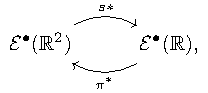
\includegraphics{sheaves-1-n-2-case}
  \]
  where \(\pi^*\) is the pullback along the projection
  \(\bbR^2\to\bbR\). It takes a form in \(x\) and treats it as a form in
  \(x,y\). The pullback along the zero section \(s^*\) sets \(y\) and
  \(dy\) to zero. Note that \(s^*\circ\pi^*\) is the identity. Although
  \(\pi^*\circ s^*\) is not the identity, we will show that it induces the
  identity on cohomology. This will show that \(H_\dR^*(\bbR^2)\cong
  H_\dR^*(\bbR)\), which is all we need. This involves a new concept. We
  introduce an operator \(H\colon\calE^p(\bbR^2)\to\calE^{p-1}(\bbR^2)\) of
  degree \(-1\) called a \emph{homotopy}. It integrates \(y\) as follows:
  \begin{align*}
    H\bigl(f(x,y)\bigr)&=0\\
    H\bigl(f(x,y)\diff x)&=0\\
    H\bigl(f(x,y)\diff y\bigr)
                       &=\int_0^y f(x,t)\diff t\\
    H\bigl(f(x,y)\diff x\wedge dy\bigr)
    &=\left[\int_0^y f(x,t)\diff t\right]dx.
  \end{align*}

  A computation using nothing more than the fundamental theorem of calculus
  shows that
  \[
    1-\pi^*s^*=\pm(Hd-dH).
  \]
  This implies that the left side induces \(0\) on \(H^*_{\dR}(\bbR^2)\),
  or equivalently \(\pi^*\circ s^*\) acts like the identity on
  cohomology.
\end{proof}

Before describing de Rham's theorem, we have to say what's happening at the
othe rend. The standard \(n\) dimensional simplex, or \(n\)-simplex,
\(\Delta^n\subset\bbR^{n+1}\) is the convex hull of the unit vectors
\((1,0,\dotsc,0),(0,1,0,\dotsc,0),\dotsc\). The convex hull of the subset of
these is called a face. This is homeomorphic to a simplex of smaller
dimension. Omitting all but the \(i\)\textsup{th} vertex is called the
\(i\)\textsup{th} face of \(\Delta^n\). We have a standard homeomorphism
\[
  \delta_i\colon\Delta^{n-1}\to\text{\(i\)\textsup{th} face of \(\Delta^n\)}.
\]

A geometric simplicial complex is given by a collection of simplices glued
along faces. Historically, the first cohomology theory was defined for
simplicial complexes. A bit later singular cohomology was developed, which
is an arbitrary topological space \(X\). A (real/complex) singular
\(p\)-cochain \(\alpha\) is an integer (real/complex) valued function on
the set of all continuous maps \(f\colon\Delta^p\to X\). It might help to
think of \(\alpha(f)\) as a combinatorial integral \(\int_f\alpha\). Let
\(S^p(X)\) (\(S^p(X,\bbR)\), \(S^p(X,\bbC)\)) denote the group of these
cochains. Define \(\delta\colon S^p(X)\to S^{p+1}(X)\) by
\[
  \delta(\alpha)(f)=\sum(-1)^i\alpha(f\circ\delta_i).
\]

\begin{lemma}
  \[\delta^2=0.\]
\end{lemma}
\begin{proof}[For \(p=0\)]
  Let \(\alpha\in S^0\). Fix \(f\colon\Delta^2\to X\). Label the
  restriction of \(f\) to the vertices by \(0,1,2\) and faces
  \(01,02,12\). Then
  \begin{align*}
    \delta^2(f)&=\delta\alpha(12)-\delta\alpha(02)+\delta\alpha(01)\\
               &=\alpha(1)-\alpha(2)-\alpha(0)+\alpha(2)+\alpha(0)-\alpha(1)\\
               &=0.
  \end{align*}
\end{proof}

Thus we have a complex. Singular cohomology is defined by
\(H^p(X,\bbZ)=H^p(S^\bullet(X),\delta)\), and similarly for real or complex
valued singular cohomology. These groups are highly computable.

\begin{theorem}[de Rham]
  If \(X\subset\bbR^n\) is open, or more generally a manifold, then
  \(H^p_\dR(X,\bbR)\cong H^p(X,\bbR)\) for all \(p\).
\end{theorem}

We will give a proof of this later on as an easy application of sheaf
theory. Sheaf methods will help obtain parallel theorems.

\begin{theorem}[Holomorphic de Rham]
  If \(X\subset\bbC^n\) is a complex manifold, then \(H^p(X,\bbC)\) can be
  computed using algebraic differential forms.
\end{theorem}

The last theorem is due to Grothendieck. The proof is a lot harder, so
we'll try to give the proof by the end of the semester, but there's no
guarantee.

\section{A crash course in homological algebra}
By the 1940s techniques from algebraic topology began to be applied to pure
algebra, giving rise to a new subject. To begin with, recall that a
category \(\scrC\) consists of a set or class of objects (e.g., sets,
groups, topological spaces) and morphisms (e.g., functions, homomorphisms,
continuous maps) between pairs of objects \(\Hom_\scrC(A,B)\). We require
an identity \(\id_A\in\Hom(A,A)\) for each object \(A\), and associative
composition law.

In this section, we will focus on one particular example. Let \(R\) be an
associative (but possibly noncommutative ring) with identity \(1\), and let
\(\RMod R\) be the category of left \(R\)-modules and homomorphisms. We
write \(\Hom_R(\blank,\blank)\) for the morphisms. It is worth noting that
\(\RMod\bbZ\) is the category of Abelian groups. These categories have the
following features:
\begin{enumerate}
\item \(\Hom_R(\blank,\blank)\) is an Abelian group, and composition is
  distributive.
\item There is a zero object \(0\) such that \(\Hom_R(0,M)=\Hom_R(M,0)=0\).
\item Every pair of objects \(A\), \(B\) has a direct sum \(A\oplus b\)
  characterized by certain universal properties.
\item Morphisms have kernels and images, characterized by the appropriate
  universal properties.
\end{enumerate}

We will encounter other categories satisfying these conditions later
on. Such categories are called Abelian. We have been a bit vague about the
precise axioms; se Weibel's Homological Algebra for this.

\subsection{Diagram Chasing}
A sequence
\[
  A\xright{f}B\xright{g}C
\]
is called \emph{exact} if \(\Ker g=\Img f\). A useful skill in this
business is to be able to prove things by diagram chasing.

\begin{exercise}
  Given a commutative diagram with exact rows
  \[
    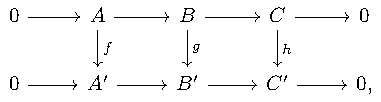
\includegraphics{exercise-2-1}
  \]
  show that \(g\) is an isomorphism if \(f\) and \(h\) are isomorphisms.
\end{exercise}
\begin{solution*}

\end{solution*}

\begin{theorem}[Snake lemma]
  If
  \[
    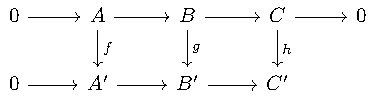
\includegraphics{snake-lemma-2}
  \]
  is a commutative diagram with exact rows, then there is an exact sequence
  \[
    0\To\Ker f
    \To\Ker g
    \To\Ker h
    \xright{\partial}\Coker f
    \To\Coker g
    \To\Coker h.
  \]
\end{theorem}
\section[\(\Hom\) Functors]{\(\boldsymbol\Hom\) Functors}
A \emph{(covariant) functor \(F\)} from one category to another is a
function taking objects to objects and morphisms to morphisms such that if
\(f\colon A\to B\) then \(F(f)\colon F(A)\to F(B)\),
\(F(\id_A)=\id_{F(A)}\), and \(F(f\circ g)=F(f)\circ F(g)\). A
contravariant functor reverses direction in the sense that
\(F(f)\colon F(B)\to F(A)\), \(F(\id_A)=\id_{F(A)}\), and
\(F(f\circ g)=F(g)\circ F(f)\). Here are two basic examples: If
\(M\in\RMod R\), then \(F(\blank)=\Hom_R(M,\blank)\) is a covariant functor
from \(\RMod R\) to \(\RMod{\bbZ}\).
\[
  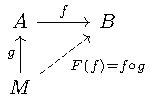
\includegraphics{mod-functor}
\]
When \(R\) is commutative, \(F(\blank)\) is naturally an \(R\)-module, but
not otherwise. Similarly, \(\Hom_R(\blank,M)\) is a contravariant functor
from \(\RMod R\) to \(\RMod\bbZ\) (or \(\RMod R\)) when \(R\) is
commutative).

\begin{lemma}
  Suppose that
  \[
    0\To A\To B\To C\To 0
  \]
  is exact. Then
  \begin{enumerate}[label=\emph{(\alph*)},noitemsep]
  \item \[0\To\Hom(M,A)\To\Hom(M,B)\To\Hom(M,C),\]
  \item \[0\To\Hom(C,M)\To\Hom(B,M)\To\Hom(A,M)\]
  \end{enumerate}
  are both exact.
\end{lemma}
The proof is straight forward and will be omitted.

\begin{exercise}
  Prove the lemma.
\end{exercise}

\begin{exercise}
  Prove that
  \[0\To\Hom(M,A)\To\Hom(M,B)\To\Hom(M,C),\]
  and
  \[0\To\Hom(C,M)\To\Hom(B,M)\To\Hom(A,M)\]
  are exact when the sequence
  \[0\To A\To B\To C\To 0\]
  is split exact. This means that there exists a map \(s\colon C\to B\),
  called a splitting, such that \(p\circ s=\id_C\).
\end{exercise}

A (contravariant) functor is called exact if it preserves exact
sequences. The lemma says that the \(\Hom\) functors have the weaker
property left exactness. They are not exact, in general:

\begin{example}
  Let \(R=\bbZ\), \(M=\bbZ/2\). Note that \(\Hom(M,\bbZ)=0\) and
  \(\Hom(M,M)=\bbZ/2\). So \(\Hom(M,\blank)\) applied to
  \[0\To\bbZ\xright{2}\bbZ\To\bbZ/2\To 0\]
  yields the sequence
  \[0\To 0\To 0\To\bbZ/2.\]
  The last map is certainly not onto.
\end{example}

%%% Local Variables:
%%% mode: latex
%%% TeX-master: "../Fall16-Notes"
%%% End:
